%%
%%	This file will gradually become a list of \input statements as the writeups for each of the proposed research
%%	methods have more work filling in each section. 
%%
%%
%%
%%
%%

\section{ALoVaS Models, the Lasso, Horseshoe, and SSVS priors}
\label{ch:proposed_futue_work}

We investigate several priors for use in variable selection with decision trees. They are: 

\begin{itemize}
\item A stochastic search approach (method of George and McCulloch and Cui and George) \cite{cui2008empirical,george1993variable}. 
\item A lasso prior on the means of the MVN, \newabbrev{abbrev:MVN} probably using parameter expansion to get Gibbs updates \cite{park2008bayesian}. 
\item A multivariate half-Cauchy prior using parameter expansion (Huang and Wand method) \cite{huang2013simple,polson2011half,carvalho2010horseshoe,carvalhohandling}. 
\item A `local' prior approach (Valen Johnson and David Rossell JRSS B 2010 approach) \cite{johnson2010use}. 
\end{itemize}

We will discuss the preliminary details of each method in sequence in this chapter. 
%\textbf{Primary contributions of this research chapter:}

\subsection{An SSVS approach to Variable Selection with Decision Trees}

Variable selection with SSVS facilitates a Bayesian approach to variable selection in decision trees. Prior methods have examined bootstrapping approaches and used some complicated math to allow the statistician to peer inside the black box method known as randomForest \cite{ishwaran2010high, ishwaran2007variable}, often with little insight or understanding. The SSVS prior allows us to ``test'' whether the constant prior probability of selecting a covariate for all dimensions is appropriate for the given dataset. This means we can test, for any dataset, whether the CGM model of covariate selection is appropriate.
%In addition we receive an explicit measure of which covariates are important, something not achieved bagging , bumping or boosting \cite{breiman1996bagging, tibshirani1999model, freund1999short}. 

We will implement and compare our method against other methods such as observed frequency, a na\"{i}ve method, as well as the maximal subtree approach of Ishwaran et al. \cite{ishwaran2010high, ishwaran2007variable}. The SSVS approach involves a prior on the normal means of the form 

\begin{equation}
\pi(\mu_i\vert \tau_i, p_i, c_i) \propto p_iN(\mu_i, \tau_i^2)+(1-p_i)N(\mu_i, c_i^2\tau_i^2).
\end{equation}

Here the $c_i >1$ and $1>\tau_i>0$ is small. Usually $p_i\equiv1/2$ but it is also possible to put a prior on these hyper-parameters. The advantage of a mixture prior in this form is that Gibbs samples are readily available for each of the desired quantities facilitating fast sampling.     

What needs to be done for this approach is a couple of things: 

\begin{itemize}
\item Determine posteriors using these forms of priors. 
\item Determine if Gibbs sampling can be done on the resulting posteriors if priors for $p_i$ and/or $c_i$ and $\tau_i$ are used. 
\item Determine if a Beta prior on $p_i$ is computationally feasible.  
\item Extensive simulation studies and hyper-parameter sensitivities.
\end{itemize}
Plus any suggestions from the committee.

\subsection{A Lasso Prior}
In this section we propose to use parameter expansion to facilitate Gibbs sampling within the sampling framework for the posterior means for each covariate in the normal space. We use the ALN transform to then convert to probabilities. 
The key idea we use for parameter expansion is the scale mixture of normals representation of a Laplace prior. This representation is stated here for reference.

If $V \sim \text{Exponential(1)}$ and $Z \sim N(0, 1)$ independent of $V$, then $X = \mu + b \sqrt{2 V}Z \sim \mathrm{Laplace}(\mu,b)$. 

Equivalently we can write this as the hierarchy

\begin{equation}\label{eqn:normal_cond_lhood_lasso}
X \vert V \sim N[\mu, \sigma^22V],
\end{equation}

\begin{equation}\newnot{symbol:exponential_dist}
V \sim \text{Exponential}(1), \text{ and}
\end{equation}

\begin{equation}\newnot{symbol:laplace_dist}
X \sim \text{Laplace}(\mu, \sigma)
\end{equation}

What we want to examine here is whether shrinkage along an $L_1$ penalty will achieve similar results to the SSVS approach and give us meaningful results. The belief here is the same as in the SSVS approach, shrinkage will shrink means toward zero in the multivariate normal. These sampled values from the multivariate normal will then be transformed into something on the $[0,1]$ (probability) scale using the ALN transform. Values of zero, or near zero, on the normal space transform into values of approximately $1/(d+1)$. The probabilities with values around $1/(d+1)$ correspond to covariates we are indifferent about. A confounding aspect of interpreting the probabilities is that they must all sum to 1. Therefore if some values are excessively small this may push all the other probabilities to be larger. If something like this happens it is then difficult to determine which covariates are non-informative. Further simulations regarding selecting covariates using the rule of Equation \ref{eqn:cov_inclusion_rule} will be conducted using the ALN transform and will be done on several simulated and real data examples.    

What needs to be done for this approach is a couple of things: 

\begin{itemize}
\item Write out the full conditionals and the Gibbs samplers for this case. 
\item Code the full conditional sampler for this method. 
\item Compare parameterizations and evaluate the sensitivity to hyper-parameter specifications. 
\item Extensive simulation studies. 
\end{itemize}
Also any suggestions by the committee.
\subsection{A Half-Cauchy or Horseshoe Prior}

The following result will be useful for parameter expansion. If 

$X\vert a \sim \mathrm{Inv-Gamma}(\nu/2, \nu/a)$ and  $a \sim \mathrm{Inv-Gamma}(1/2,A^2)$, then $\sqrt{X}\sim \mathrm{Half-Cauchy}$. 

\begin{align*}
f(x) &= \int_0^\infty \underbrace{  \frac{\nu^{\nu/2}}{a^{\nu/2}\Gamma(\nu/2)x^{(\nu/2)+1}}\exp{(-\frac{\nu}{ax})}   }_{=f(x\vert a)} \underbrace{\frac{\exp{(-\frac{1}{aA^2})}}{A\sqrt{\pi}a^{3/2}}}_{=f(a)} da\\
&=\frac{\nu^{\nu/2}}{A\sqrt{\pi}\Gamma(\nu/2)x^{(\nu+2)/2}}\underbrace{\int_0^\infty a^{-\nu/2-1/2-1}\exp{(-(1/a)(\nu/x+1/A^2))}da}_{=\text{Inv-Gamma kernel}}\\
&=\frac{\nu^{\nu/2}\Gamma((\nu+1)/2)}{A\sqrt{\pi}\Gamma(\nu/2)x^{(\nu+2)/2}(\nu/x+1/A^2)^{(\nu+1)/2}}\\
&\propto \frac{1}{\sqrt{x}x^{(\nu+1)/2}(\nu/x+1/A^2)^{(\nu+1)/2}}\\
& =\frac{1}{\sqrt{x}(\nu+x/A^2)^{(\nu+1)/2}  }\\
&=\frac{1}{\sqrt{x}(\nu+x/A^2)^{(\nu+1)/2}  }.
\end{align*}

Making the change of variable $x=y^2$, which implies $dx/(2\sqrt{x})=dy$, shows us that 

\begin{equation}
f(y) \propto (1+(y/A)^2/\nu)^{-(\nu+1)/2},
\end{equation}
for $y>0$ which is the definition of a half-Cauchy density. 

Huang and Wand \cite{huang2013simple} indicate that using an inverse-Wishart prior on the variances, with each standard deviation having a half-Cauchy prior, gives a scaled beta marginal for each correlation. At this point it is worth recalling that the t and half-t distributions have as special cases, the Cauchy and half-Cauchy distributions when the degrees of freedom parameter ($\nu$) in the t and half-t is set to $\nu=1$. We will use the scale mixture representation of inverse gammas given above to put half-Cauchy priors on the standard deviations.  


%%%% Leave this chunk in for now, but will probably cut it in the end
The hierarchical model for the sparse inverse-Wishart prior as

\begin{equation}\newnot{symbol:inv_wishart}
\Sigma\vert a_1, \dots,a_p \sim \text{Inv-Wishart}(\nu+p-1, 2\nu\text{diag}(1/a_1,\dots,1/a_p)), 
\end{equation} 

\begin{equation}
a_k \sim i.i.d.\ \text{Inverse-Gamma}(1/2,1/A_k^2),
\end{equation} 
for $k=1,\dots,p$.  
The inverse-Wishart has the density 
\begin{equation}
p(\Sigma \vert \kappa, \text{B})\propto \vert \text{B}\vert^{\kappa/2}\vert\Sigma\vert^{-(\kappa+p+1)/2}\exp{(-\frac{1}{2}\text{tr}(B\Sigma^{-1}))}.
\end{equation}
\newnot{symbol:trace}
Huang and Wand \cite{huang2013simple} argue that this model constitutes a matrix generalization of the half-t$(\nu, A_k)$ prior for each standard deviation term, and also allows for uniform marginal distributions on each correlation parameter in $\Sigma$, by choosing $\nu=2$. If one instead chooses $\nu=1$, this corresponds to a $S\beta(\rho;1/2,1/2,-1,1)$ distribution. This half-t prior works well in their simulations for both correlated covariates and non-correlated covariates.  
%%%% End of this chunk in for now, but will probably cut it in the end
What needs to be done for this method is: 

\begin{itemize}
\item Write down full conditionals.
\item Code the full conditionals samplers. 
\item Determine the dimensionality in which this method is feasible and if that is useful for our problems.
\item Extensive simulation studies. 
\end{itemize}
Also, any suggestions that committee brings up during the proposal.

%\subsection{A Local Prior Approach}
%
%Another alternative we will examine is a `local' prior approach using a moment prior defined in Johnson and Rossell \cite{johnson2010use}. These moment priors are functions that have densities that look like those in Figure \ref{fig:local_priors}.
%
%\begin{figure}[h]
%  \centering
%    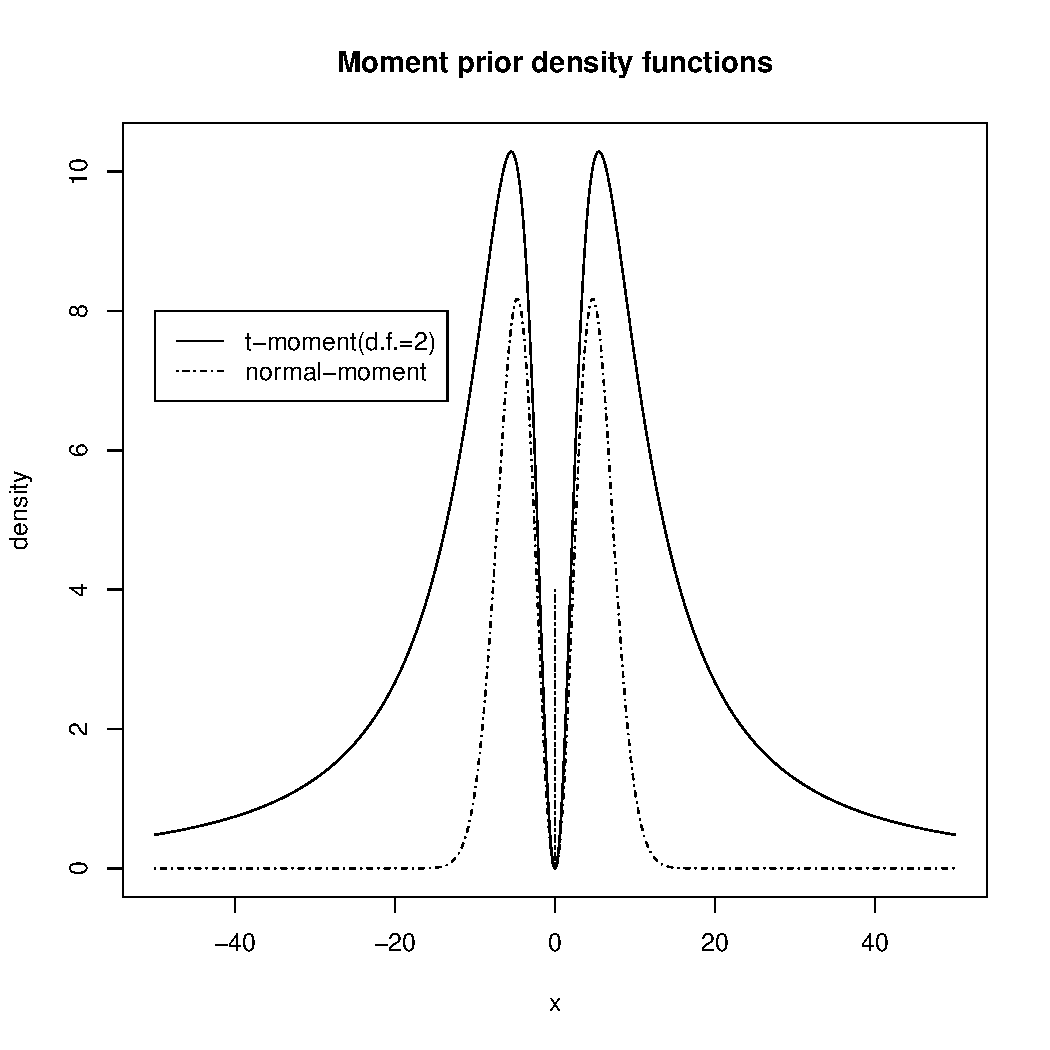
\includegraphics[width=0.7\textwidth]{moment_prior_plot_BW.pdf}
%    \caption[Local priors with a point mass at 0]{Local priors with a point mass at 0.}
%  \label{fig:local_priors}
%\end{figure}
%
%The moment priors are defined by the densities 
%
%\begin{equation}
%f_k(x)\propto (x-\mu)^{2k}\pi(x-\mu),
%\end{equation}
%where here $\mu$ denotes the first moment and $k$ is a specified constant. In Figure \ref{fig:local_priors} $k=1$, $\mu=0$, and the two $\pi(x)$s represent a normal and a t distribution with degrees of freedom $2$. The basic idea with the local priors is that we want to circumvent the necessity of specifying informative prior means for the normal priors. These moment priors have large probability masses on two regions, a negative region and a positive region. The two local modes allow the priors' means to encourage the selection of certain covariates (in the positive mode) and to discourage the selection of other covariates (in the negative mode).
%
%What needs to be done for this approach is extensive simulation studies and hyper-parameter sensitivities.
%
%Also, any suggestions that committee brings up during the proposal.
